\documentclass[12pt,a4paper,twoside]{book} 
\usepackage[spanish]{babel} % de pedro
\usepackage{graphics,graphicx,epsfig,color,float,afterpage,fancyheadings,subfigure,moreverb,alltt} % de pedro
\usepackage[latin1]{inputenc} % tildes de pedro

\usepackage{algorithm}
\usepackage{algorithmic}

\usepackage{rotating}
\usepackage{url}

%% Esta letra se convierte mejor a pdf que la normal
\usepackage{ae}

%%% Para las fuentes matemticas
\usepackage{amsfonts}

\usepackage{subfigure}

\usepackage{pstricks} % para los dibujos del da
\usepackage{lscape} % para las pginas en horizontal
\usepackage{portland} % para las pginas en horizontal
\usepackage{supertabular} % para las tablas de ms de una pgina
\usepackage{tabularx} % para las tablas del tipo tabularx
%\usepackage{glossary}
%\documentclass[a4paper,spanish,12pt]{book} % esto es de gustavo
%\usepackage{amsmath,amsfonts}   % underset mathbb
%\usepackage{authordate1-4}      % bib style
%\usepackage{epsfig}     % eps
\usepackage{epic}           % graficos
%\usepackage{eepic}           % graficos
\usepackage{curvesls}           % curvas
\usepackage{amssymb}
%\usepackage{fancyheadings}  % encabezados
%\usepackage{hhline}             % hhline
%\usepackage[latin1]{inputenc}   % tildes
%\usepackage{makeidx}        % ndices
%\usepackage{setspace}           % interlinea
%\usepackage[spanish]{babel} % espaol

%%%%%%%%%%%%%%%%%%%%%%%%%%%%%%%%%%%%%%%%%%%%%%%%%%%%%%%%%%%%%%%%%%%%%%%%%%%%%%%

\author{juanlu}
\title{Tesis de Juan Lus Jimnez Laredo}




\newcommand{\fecha}{\footnotesize{[ Impreso: \the\day-\ifcase\month\or
    Ene\or Feb\or Mar\or Abr\or May\or Jun\or Jul\or Ago\or Sep\or
      Oct\or Nov\or Dic\fi-\the\year ]}}

\newcommand{\N}{\mathbb{N}}

%% Para corregir las cabeceras largas
\newcommand{\cabecera}[2]{
\markright{\ref{#1}. \hspace{0.1ex} \MakeUppercase{#2}}}


%\pagestyle{headings}
%\renewcommand{\chaptermark}[1]{\markboth{\fecha \\ \\ #1}{}}
%\renewcommand{\sectionmark}[1]{\markright{#1 \\ \\ \fecha}}
%\addtolength{\headheight}{2.5pt}



%\lhead[\it\thechapter]{\sl\rightmark}
%\rhead[\rm\leftmark]{\it\thesection}
%\rfoot[]{\thepage}
%\cfoot[]{}
%\lfoot[\thepage]{}

%\thispagestyle{plain}

\setcounter{secnumdepth}{3}
\setcounter{tocdepth}{3}

%\renewcommand{\baselinestretch}{1.2}
%\setlength{\parskip}{0.8ex}

\newtheorem{theorem}{\sf Teorema}
\newtheorem{lemma}{\sf Lema}

\newcommand{\rem}[1]{\S\iffalse #1 \fi}
\newcommand{\cur}[1]{ {\it #1\/} }
\newcommand{\crcl}[1]{#1\kern-9pt\raise1pt\hbox{$\bigcirc$}}
\newcommand{\evag}{{\sf EvAg}}
\newcommand{\evagp}{{\sf EvAg.}}
\newcommand{\evags}{{\sf EvAgs}}
\newcommand{\evagsp}{{\sf EvAgs.}}

\newcommand{\prog}[2] {
   \small
   \begin{minipage}[t]{75mm} {\tt #1}  \end{minipage}
   \begin{minipage}[t]{60mm} {#2}      \end{minipage}
   \\
}
\newcommand{\prg}[2] { {\tt #1} & {\sf #2} \\}

\newcommand{\wmfspecial}[4]{
   \begin{figure}[h]
   \centerline{\psfig{figure=#1,height=#2}}
   \caption{#3}   \label{#4}
   \end{figure}
}                   % USO: \wmfspecial{nombre.eps}{altura}{leyenda}{etiqueta}

\def\stackunder#1#2{\mathrel{\mathop{#2}\limits_{#1}}}

\def\marco #1#2#3#4{\centerline{       % USO: \marco{.1}{10}{124mm}
  \vbox{\hrule height #1pt%
  \hbox{\vrule width #1pt\kern #2pt%
  \vbox{\kern #2pt%
  \vbox{\hsize #3\noindent #4}%
  \kern #2pt}%
  \kern #2pt\vrule width #1pt}%
  \hrule height0pt depth #1pt}} }


\newcommand{\symnote}[2]{\symbolnote{#1}{#2}}

\newfont{\bi}{cmbxti10 scaled\magstep1}       % bf + it


%% Ruta de las figuras
\graphicspath{{../figuras/}}


\begin{document}
           % Eliminarlo al compilar el documento maestro, ponerlo para compilarlo separado

%%%%%%%%%%%%%%%%%%%%%%%%%%%%%%%%%%%%%%%%%%%%%%%%%%%%%%%%%%%%%%%%%%%%%%%%%%%%%%%
%%                                                                           %%
%%                             Tesis Doctoral:                               %%
%%                        Juan Luis Jimenez Laredo                           %%
%%                                                                           %%
%%%%%%%%%%%%%%%%%%%%%%%%%%%%%%%%%%%%%%%%%%%%%%%%%%%%%%%%%%%%%%%%%%%%%%%%%%%%%%%

%\cabecera{cap:p2pea}{Peer-to-Peer Evolutionary Algorithms}  %Descomentarlo para compilar maestro
\chapter{\textit{Peer-to-Peer Evolutionary Algorithms}}
\label{cap:p2pea}
%\cabecera{cap:p2pea}{Peer-to-Peer Evolutionary Algorithms} %Descomentarlo para compilar maestro
%%%%%%%%%%%%%%%%%%%%%%%%%%%%%%%%%%%%%%%%%%%%%%%%%%%%%%%%%%%%%

%%%%%%%%%%%%%%%%%%%%%%%%%%%%%%%%%%%%%%%%%%%%%%%%%%%%%%%%%%%%%
\section{Background}
%%%%%%%%%%%%%%%%%%%%%%%%%%%%%%%%%%%%%%%%%%%%%%%%%%%%%%%%%%%%%

%%%%%%%%%%%%%%%%%%%%%%%%%%%%%%%%%%%%%%%%%%%%%%%%%%%%%%%%%%%%%
\section{P2P systems}
%%%%%%%%%%%%%%%%%%%%%%%%%%%%%%%%%%%%%%%%%%%%%%%%%%%%%%%%%%%%%
DHT, gnutella, JXTA...


%%%%%%%%%%%%%%%%%%%%%%%%%%%%%%%%%%%%%%%%%%%%%%%%%%%%%%%%%%%%%
\section{P2P applications}
%%%%%%%%%%%%%%%%%%%%%%%%%%%%%%%%%%%%%%%%%%%%%%%%%%%%%%%%%%%%%
Probably the most interesting field where EAs on P2P could be applied is on solving Dynamic function optimization problems where problems optima vary in time. Some examples are related with processes such as task-scheduling or controlling traffic-lights systems.
    Within this context, decentralized monitored systems require a special attention. Our proposal would report the benefits of spreading the monitored data among the network in a P2P fashion (what is interesting on the recalculation fitness process) while the dEA would be optimizing the dynamic function by taking advantage of the available resources (which could go from a MANET of sensors to a decentralized weather forecasting system).
    As conclusion, EA on P2P could be integrated on corporative ERPs while  exploding their idle resources and optimizing a dynamic problem.


%%%%%%%%%%%%%%%%%%%%%%%%%%%%%%%%%%%%%%%%%%%%%%%%%%%%%%%%%%%%%
\section{P2P issues}
%%%%%%%%%%%%%%%%%%%%%%%%%%%%%%%%%%%%%%%%%%%%%%%%%%%%%%%%%%%%%

\subsection{Scalability}
Since our model is expected to work on distributed hardware one of its main foundations should be to obtain reasonable speed-up with respect to the use of a single machine.
Concerning Eas speed-up, scalability depends directly on the population size and the parallelization grain. As bigger the population size and finer the grain as bigger the number of nodes can be involved into an experiment, increasing the speed-up. A main subject is taking into account that the population size affects the algorithm and a balance should be kept between speed-up and algorithmic results.
Orthogonally, nodes can be understood as virtual nodes. A load balance mechanism should deal with the performance by balancing the virtual nodes among the available physical nodes.

\subsection{Fault Tolerance}
\subsection{Bootstrapping}
\subsection{Heterogeneity}

%%%%%%%%%%%%%%%%%%%%%%%%%%%%%%%%%%%%%%%%%%%%%%%%%%%%%%%%%%%%%
\section{State of the art in Peer-to-Peer Evolutionary Computing: Adventages and drawbacks}
%%%%%%%%%%%%%%%%%%%%%%%%%%%%%%%%%%%%%%%%%%%%%%%%%%%%%%%%%%%%%

\subsection{DREAM}

\subsection{SOTEA}

\subsection{P-CAGE}

%%%%%%%%%%%%%%%%%%%%%%%%%%%%%%%%%%%%%%%%%%%%%%%%%%%%%%%%%%%%%
\section{Population structure as a complex network}
%%%%%%%%%%%%%%%%%%%%%%%%%%%%%%%%%%%%%%%%%%%%%%%%%%%%%%%%%%%%%


To help understand the role of the population structure in a P2P EA, this section introduces the structural design of a simple and easy understandable complex network proposed in \cite{wattsstrogatz}. As described by the authors, the procedure for building a small-world topology can start from a ring lattice with $n$ vertices and $k$ edges per vertex. With a given probability $p$, each edge is rewired at random. Since the procedure does not allow duplicate edges, no edge is generated whenever it matches an existing one. This way for a rewiring factor of
$p=0$ the ring lattice is kept while for $p=1$ a random graph is generated. It has been shown that already for small values of $p$, the average distance between two nodes decreases rapidly. 


\begin{figure*}[htbp]
\centerline{\subfigure{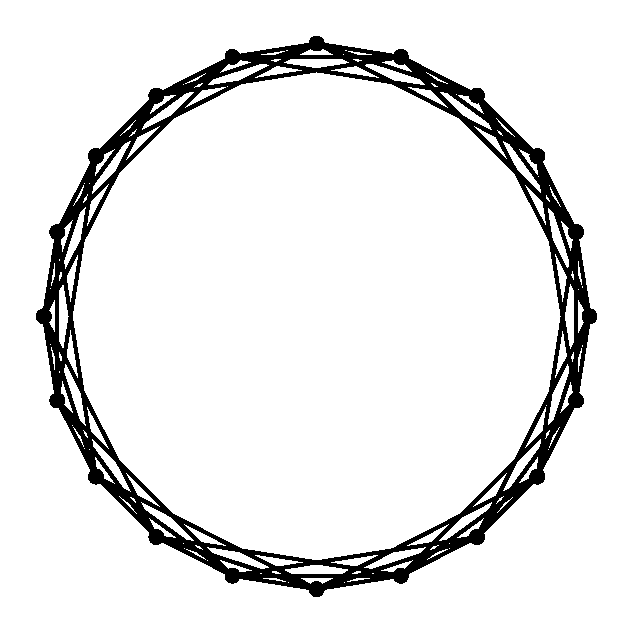
\includegraphics[width=1.5in]{WS-20-0000}
}
\hfil
\subfigure{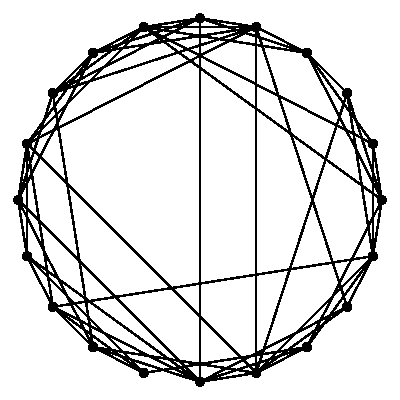
\includegraphics[width=1.5in]{WS-20-0200}
}
\hfil
\subfigure{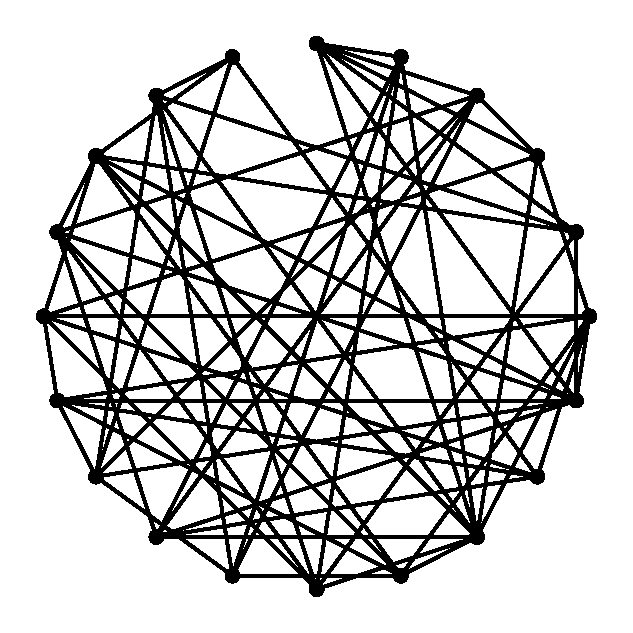
\includegraphics[width=1.5in]{WS-20-1000}
}}
\caption{Watts-Strogatz graphs with $n=20$ and $k=6$. From left to right, the original ring lattice for $p=0$, a small-world graph for $p=0.2$ and a random graph for $p=1$. 
}
\label{fig:small-world}
\end{figure*}


Figure \ref{fig:small-world} shows three instances of the Watts-Strogatz model in which the small-world graph preserves the high clustering coefficient of regular lattices and the small average path length of random graphs. Despite having a larger average path length than panmictic graphs, the inhomogeneity in such kind of topologies was shown in \cite{giacobini:gecco05} to induce qualitatively similar selection pressures on EAs compared to panmictic population structures. 

The influence  in the environmental selection pressure of such population structures can be represented by their takeover time curves. \cite{Goldberg91acomparative} defines the takeover time as the time that it takes for a single, best individual to take over the entire population without any other mechanism than selection. Hence, takeover time is the proportion of best individuals formulated as a function of time. 






\begin{figure*}[htbp]
\centerline{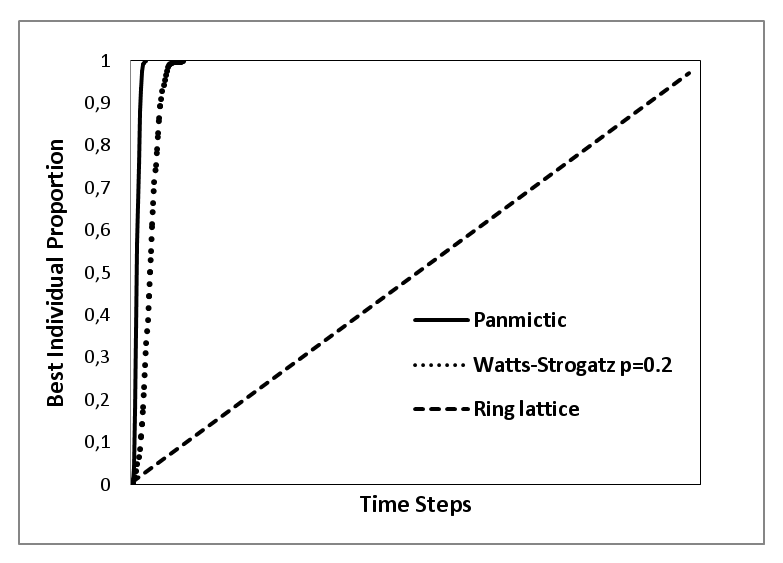
\includegraphics[width=2.5in]{takeoverwattsstrogatz}}
\caption{Takeover time curves in a panmictic graph, Watts-Strogatz graph with $p=0.2$ and the original ring lattice with $k=2$. All results for $n=1600$ and binary tournament. }
\label{fig:takeoversw}
\end{figure*}

Figure \ref{fig:takeoversw} shows that the takeover time curve in the Watts-Strogatz graph is similar to a panmictic graph meaning that the induced selection pressures with both topologies are roughly equivalent. As in Watts-Strogatz small-world topologies, this paper shows that P2P topologies can induce similar selection pressures to the panmictic one, allowing in addition a better scalability behaviour at the lower edge cardinality of P2P systems.

%%%%%%%%%%%%%% Bibliografia %%%%%%%%%%%%%%%

\bibliographystyle{alpha}  % Eliminarlo al compilar el documento maestro, ponerlo para compilarlo separado
\bibliography{p2pea}% Eliminarlo al compilar el documento maestro, ponerlo para compilarlo separado

\end{document}             % Eliminarlo al compilar el documento maestro, ponerlo para compilarlo separado
